% !TEX root = saveliev_physics_general_course_1.tex
%!TEX TS-program = pdflatex
%!TEX encoding = UTF-8 Unicode


\chapter{OSCILLATORY MOTION}\label{chap:7}

\section{General}\label{sec:7_1}

Oscillations are defined as processes distinguished by a certain degree of repetition. For example, the swings of a clock pendulum, the vibrations of a string or the leg of a tuning fork, and the voltage across the plates of a capacitor in a radio receiver circuit have this property of repetition.

Depending on the physical nature of the repeating process, we distinguish mechanical, electromagnetic, sound, and other oscillations. In the present chapter, we shall deal with mechanical oscillations.

Oscillations (vibrations) are widespread in nature and engineering. They often have a negative influence. The oscillations of a railway bridge due to the impacts imparted to it by the wheels of a train passing over the rail joints, the vibrations of a ship's hull caused by rotation of the propeller, the vibrations of the wings of an aircraft are all processes that may have catastrophic consequences. The task in such cases is to prevent the setting up of oscillations or at any rate to prevent them from reaching dangerous magnitudes.
Oscillatory processes are also at the very foundation of various branches of engineering. For instance, radio engineering owes its very existence to oscillatory processes. Depending on the nature of the action on an oscillating system, we distinguish free (or natural) oscillations, forced oscillations, auto-oscillations, and parametric oscillations.

\textbf{Free} or \textbf{natural oscillations} occur in a system left alone after an impetus was imparted to it or it was brought out of the equilibrium position. An example are the oscillations of a ball suspended on a string (a pendulum). To initiate oscillations, we may either push the ball or move it to a side and release it. 

In \textbf{forced oscillations}, the oscillating system is acted upon by an external periodically changing force. An example here are the oscillations of a bridge set up when people walking in step pass over it.

\textbf{Auto-oscillations}, like forced ones, are attended by the action of external forces on the oscillating system, but the moments of time when these actions are exerted are set by the oscillating system itself---the latter controls the external action. Examples of an auto-oscillating system are clocks in which a pendulum receives pushes at the expense of the energy of a lifted weight or a coiled spring, and these pushes occur when the pendulum passes through its middle position.

In \textbf{parametric oscillations}, external action causes periodic changes in a parameter of a system, for instance, in the length of a thread on which an oscillating ball is suspended.

\textbf{Harmonic oscillations} are the simplest ones. These are oscillations when the oscillating quantity (for example, the deflection of a pendulum) changes with time according to a sine or cosine law. This kind of oscillations is especially important for the following reasons: first, oscillations in nature and engineering are often close to harmonic ones in their character, and, second, periodic processes of a different form (with a different time dependence) can be represented as the superposition of several harmonic oscillations.

\section{Small-Amplitude Oscillations}\label{sec:7_2}

Let us consider a mechanical system whose position can be set with the aid of a single quantity which we shall designate $x$. The system is said to have one degree of freedom in such cases. The angle measured from a certain plane, or the distance measured along a given curve, in particular a straight line, etc. may be the quantity $x$ determining the position of the system. The potential energy of the system will be a function of the single variable $x$: $E_{\text{p}}=E_{\text{p}}(x)$. Assume that the system has a position of stable equilibrium. In this position, the function $E_{\text{p}}(x)$ has a minimum (see Sec.~\ref{sec:3_9}). We shall measure the coordinate $x$ and the potential energy $E_{\text{p}}$ from the position of equilibrium. Hence $E_{\text{p}}(0)=0$. 

Let us expand the function $E_{\text{p}}(x)$ in a power series and consider only small-amplitude oscillations, so that the higher powers of $x$ may be disregarded. According to the Maclaurin theorem
\begin{equation*}
	E_{\text{p}}(x) = E_{\text{p}}(0) + E_{\text{p}}'(0)\,x + \frac{1}{2}E_{\text{p}}''(0)\,x^2
\end{equation*}

\noindent
(owing to the small value of $x$ we disregard the remaining terms). Since $E_{\text{p}}(x)$ at $x=0$ has a minimum, then $E_{\text{p}}'(0)$ equals zero, and $E_{\text{p}}''(0)$ is positive. In addition, according to our condition, $E_{\text{p}}(0)=0$. Let us introduce the symbol $E_{\text{p}}''(0)=k$ (where $k>0$). Hence,
\begin{equation}\label{eq:7_1}
	E_{\text{p}}(x) = \frac{1}{2}kx^2.
\end{equation}

Equation~\eqref{eq:7_1} is identical with \eqn{3_78} for the potential energy of a deformed spring. Using \eqn{3_32}, let us find the force acting on the system:
\begin{equation}\label{eq:7_2}
	F_x = -\diffpartial{E_{\text{p}}}{x} = -kx.
\end{equation}

This equation gives the projection of the force onto the direction $x$. In the following, we shall omit the subscript $x$ in designating the force, \ie, we shall write \eqn{7_2} in the form $F=-kx$.

Equation~\eqref{eq:7_2} is identical with \eqn{2_26} for the elastic force of a deformed spring. This is why forces of the kind shown by \eqn{7_2} regardless of their nature, are called \textbf{quasi-elastic}. It is easy to see that a force described by \eqn{7_2} is always directed toward the position of equilibrium. The magnitude of the force is proportional to the deviation of the system from its equilibrium position. A force having such properties is sometimes defined as a \textbf{restoring force}.

\begin{figure}[t]
	\begin{center}
		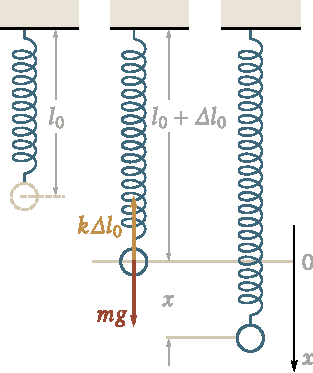
\includegraphics[scale=0.95]{figures/cap_07/fig_7_1.pdf}
		\caption[]{}
		\label{fig:7_1}
	\end{center}
	\vspace{-0.7cm}
\end{figure}

Let us consider as an example a system consisting of a ball of mass $m$ suspended on a spring whose mass may be ignored in comparison with $m$ (\fig{7_1}). In the equilibrium position, the force $mg$ is balanced by the elastic force $k\Delta l_0$:
\begin{equation}\label{eq:7_3}
	mg = k\Delta l_0
\end{equation}

\noindent
($\Delta l_0$ is the elongation of the spring). We shall characterize the displacement of the ball from its equilibrium position by the coordinate $x$ with the $x$-axis directed vertically downward and the zero of the axis coinciding with the position of equilibrium of the ball. If we shift the ball to the position characterized by the coordinate $x$, then the elongation of the spring will become equal to $\Delta l_0+x$, and the projection of the resultant force onto the $x$-axis will acquire the value $F=mg-k(\Delta l_0+x)$. Taking into account condition~\eqref{eq:7_3}, we find that
\begin{equation}\label{eq:7_4}
	F = -kx.
\end{equation}

\noindent
Thus, in the example considered, the resultant of the force of gravity and of the elastic force has the nature of a quasi-elastic force.

Let us impart the displacement $x=a$ to the ball and then leave the system alone. Under the action of the quasi-elastic force, the ball will move toward its equilibrium position with the constantly growing velocity $v=\dot{x}$: The potential energy of the system will diminish (\fig{7_2}), but a constantly growing kinetic energy $E_{\text{k}}=m\dot{x}^2/2$ will appear instead (we disregard the mass of the spring).

\begin{figure}[t]
	\begin{center}
		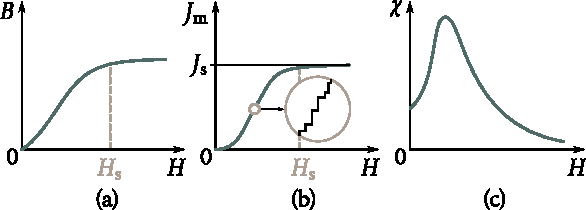
\includegraphics[scale=0.95]{figures/cap_07/fig_7_2.pdf}
		\caption[]{}
		\label{fig:7_2}
	\end{center}
	\vspace{-0.7cm}
\end{figure}

Arriving at its equilibrium position, the ball continues to move by inertia. This motion will be retarded and will stop when the kinetic energy completely transforms into potential energy, \ie, when the displacement of the ball becomes equal to $-a$. Next the same process will repeat when the ball moves in the reverse direction. If friction is absent in the system, its energy should be conserved, and the ball will move within the limits from $x=a$ to $x=-a$ for an infinitely long time.

The equation of Newton's second law for the ball is
\begin{equation}\label{eq:7_5}
	m\ddot{x} = -kx.
\end{equation}

\noindent
Introducing the symbol
\begin{equation}\label{eq:7_6}
	\omega_0^2 = \frac{k}{m}
\end{equation}

\noindent
we can transform \eqn{7_5} as follows:
\begin{equation}\label{eq:7_7}
	\ddot{x} + \omega_0^2 x = 0.
\end{equation}

\noindent
Since $k/m>0$, then $\omega_0$ is a real quantity.

Thus, in the absence of forces of friction, motion under the action of a quasi-elastic force is described by the differential equation~\eqref{eq:7_7}.

Any real oscillatory system contains resistance or damping forces whose action leads to diminishing of the energy of the system. If the depletion of the energy is not replenished as a result of the work of external forces, the oscillations will be damped. In the simplest and also the most frequently encountered case, the damping force $F^*$ is proportional to the magnitude of the velocity:
\begin{equation}\label{eq:7_8}
	F_x^* = -r\dot{x}.
\end{equation}

\noindent
Here $r$ is a constant called the \textbf{resistance coefficient}. The minus sign is due to the circumstance that the force $\vec{F}^*$ and the velocity $\vec{v}$ have opposite directions, consequently, their projections onto the $x$-axis have opposite signs.

The equation of Newton's second law when damping forces are present has the form
\begin{equation}\label{eq:7_9}
	m\ddot{x} = -kx - r\dot{x}.
\end{equation}

\noindent
Introducing the notation
\begin{equation}\label{eq:7_10}
	2\beta = \frac{r}{m}
\end{equation}

\noindent
and using \eqn{7_6}, we can write \eqn{7_9} as follows:
\begin{equation}\label{eq:7_11}
	\ddot{x} + 2\beta\dot{x} + \omega_0^2 x = 0.
\end{equation}

\noindent
This differential equation describes the damping oscillations of a system.

The oscillations described by Eqs.~\eqref{eq:7_7} and~\eqref{eq:7_11} are free (or natural): a system brought out of its equilibrium position or having received an impetus performs oscillations when left alone. Now assume that an oscillatory system experiences an external force that changes with time according to a harmonic law:
\begin{equation}\label{eq:7_12}
	F_x = F_0 \cos\omega t.
\end{equation}

\noindent
In this case, the equation of Newton's second law has the form
\begin{equation*}
	m\ddot{x} = -kx - r\dot{x} + F_0 \cos\omega t.
\end{equation*}

\noindent
Using Eqs.~\eqref{eq:7_6} and~\eqref{eq:7_10}, let us write this equation as follows:
\begin{equation}\label{eq:7_13}
	\ddot{x} + 2\beta\dot{x} +\omega_0^2 x = f_0 \cos\omega t
\end{equation}

\noindent
where
\begin{equation}\label{eq:7_14}
	f_0 = \frac{F_0}{m}.
\end{equation}

\noindent
Equation~\eqref{eq:7_13} describes forced oscillations.

We have established that when studying various kinds of oscillations we are confronted with the need to solve differential equations of the form
\begin{equation}\label{eq:7_15}
	\ddot{x} + a\dot{x} +bx = f(t)
\end{equation}

\noindent
where $a$ and $b$ are constants, and $f(t)$ is a function of $t$. An equation such as~\eqref{eq:7_15} is called a \textbf{linear differential equation with constant coefficients}. For \eqn{7_7}, we have $a=0$ and $b=\omega_0^2$ and for \eqn{7_11}, we have $a=2\beta$ and $b=\omega_0^2$. In both cases, the function $f(t)$ identically equals zero: $f(t)\equiv 0$. For forced oscillations, $f(t)=f_0\cos\omega t$.

The solution of \eqn{7_15} is greatly facilitated if we pass over to complex quantities. This is why we shall stop to briefly treat complex numbers and methods of solving linear differential equations with constant coefficients.

\section{Complex Numbers}\label{sec:7_3}

The complex number $z$ is defined as a number of the kind
\begin{equation}\label{eq:7_16}
	z = x + iy
\end{equation}

\noindent
where $x$ and $y$ are real numbers, and $i$ is imaginary unity ($i^2=-1$). The number $x$ is called the \textbf{real part} of the complex number $z$. This is written symbolically\footnote{Another form of symbolically represent the real and imaginary parts of a complex number is: $\mathrm{Re}\{z\}$ and $\mathrm{Im}\{z\}$.} in the form $x=\Re\{z\}$. The number $y$ is the \textbf{imaginary part} of $z$ (symbolically $y=\Im\{z\}$). The number
\begin{equation}\label{eq:7_17}
	z^* = x - iy
\end{equation}

\noindent
is called the \textbf{complex conjugate} of the number $x+iy$. 

The real number $x$ can be depicted by a point on the $x$-axis. The complex number $z$ can be depicted by a point on a plane with the coordinates $x$ and $y$ (\fig{7_3}). Each point of the plane corresponds to a complex number $z$. Consequently, a complex number can be given in the form of \eqn{7_16} with the aid of the Cartesian coordinates of the relevant point. The same number, however, can be given with the aid of the polar coordinates $\rho$ and $\varphi$. The following relations exist between the two pairs of coordinates:
\begin{equation}\label{eq:7_18}
	\begin{cases}
		x = \rho\cos\varphi,\quad\quad\quad y = \rho\sin\varphi,\\
		\rho = \left(x^2+y^2\right)^{1/2},\quad \varphi = \arctan\dfrac{y}{x}.
	\end{cases}
\end{equation}

The distance from the origin of coordinates to the point depicting the number $z$ is called the \textbf{absolute value} or \textbf{modulus} of the complex number (its symbol is $|z|$). It is obvious that
\begin{equation}\label{eq:7_19}
	|z| = \rho = \left(x^2+y^2\right)^{1/2}.
\end{equation}

\noindent
The quantity $\varphi$ is called the \textbf{argument} of the complex number $z$.

With a view to Eqs.~\eqref{eq:7_18}, we can write a complex number in the trigonometric form:
\begin{equation}\label{eq:7_20}
	z = \rho(\cos\varphi + i\sin\varphi).
\end{equation}

Two complex numbers $z_1=x_1+iy_1$ and $z_2=x_2+iy_2$ are considered to equal each other if their real and imaginary parts are separately equal, namely,
\begin{equation}\label{eq:7_21}
	z_1 = z_2\,\, \text{if}\,\, x_1 = x_2\,\, \text{and}\,\, y_1 = y_2.
\end{equation}

\noindent
The moduli of two equal complex numbers are identical, while their arguments can differ only in an addend that is a multiple of $2\pi$:
\begin{equation}\label{eq:7_22}
	\rho_1 = \rho_2,\quad \varphi_1 = \varphi_2\pm 2k\pi
\end{equation}

\noindent
where $k$ is an integer.

\begin{figure}[t]
	\begin{center}
		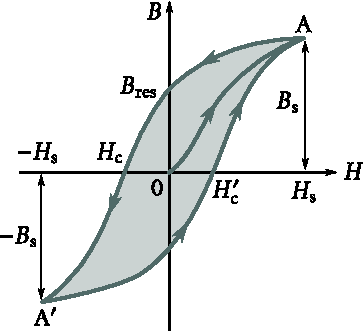
\includegraphics[scale=0.95]{figures/cap_07/fig_7_3.pdf}
		\caption[]{}
		\label{fig:7_3}
	\end{center}
	\vspace{-0.7cm}
\end{figure}

Examination of Eqs.~\eqref{eq:7_16} and~\eqref{eq:7_17} shows that when $z^*=z$, the imaginary part of $z$ vanishes, \ie, the number $z$ is a pure real number. Thus, the condition for the number $z$ being real can be written in the form
\begin{equation}\label{eq:7_23}
	z^* = z.
\end{equation}

The relation
\begin{equation}\label{eq:7_24}
	e^{i\varphi} = \cos\varphi + i\sin\varphi
\end{equation}

\noindent
is proved in mathematics and is called the \textbf{Euler formula}. Substituting $-\varphi$ for $\varphi$ in this equation and bearing in mind that $\cos(-\varphi)=\cos\varphi$ and $\sin(-\varphi)=-sin\varphi$ we get
\begin{equation}\label{eq:7_25}
	e^{-i\varphi} = \cos\varphi - i\sin\varphi.
\end{equation}

Let us summate Eqs.~\eqref{eq:7_24} and~\eqref{eq:7_25} and solve the resulting equation relative to $\cos\varphi$. We obtain
\begin{equation}\label{eq:7_26}
	\cos\varphi = \frac{1}{2}\left(e^{i\varphi} + e^{-i\varphi}\right).
\end{equation}

\noindent
Subtraction of \eqn{7_25} from~\eqref{eq:7_24} yields $\sin\varphi=\left(e^{i\varphi} + e^{-i\varphi}\right)/2i$.

Equation~\eqref{eq:7_24} can be used to write a complex number in the exponential form:
\vspace{-12pt}
\begin{equation}\label{eq:7_27}
	z = \rho e^{i\varphi}
\end{equation}

\noindent
[see \eqn{7_20}]. The complex conjugate number in the exponential form is
\begin{equation}\label{eq:7_28}
	z^* = \rho e^{-i\varphi}.
\end{equation}

\noindent
In the addition of complex numbers, their real and imaginary parts are added separately:
\begin{equation}\label{eq:7_29}
	z_1 + z_2 = (x_1 + x_2) + i(y_1 + y_2).
\end{equation}

It is convenient to multiply complex numbers by taking them in the exponential form:
\begin{equation}\label{eq:7_30}
	z = z_1 z_2 = \rho_1 e^{i\varphi_1} \rho_2 e^{i\varphi_2} = \rho_1\rho_2 e^{i(\varphi_1 + \varphi_2}.
\end{equation}

\noindent
The moduli of the complex numbers in this case are multiplied, and the arguments are added:
\begin{equation}\label{eq:7_31}
	\rho = \rho_1\rho_2,\quad \varphi = \varphi_1 + \varphi_2.
\end{equation}

\noindent
Complex numbers are divided in a similar way:
\begin{equation}\label{eq:7_32}
	z = \frac{z_1}{z_2} = \frac{\rho_1 e^{i\varphi_1}}{\rho_2 e^{i\varphi_2}} = \frac{\rho_1}{\rho_2}e^{i(\varphi_1 - \varphi_2}.
\end{equation}

It is a simple matter to find from Eqs.~\eqref{eq:7_27} and~\eqref{eq:7_28} that
\begin{equation}\label{eq:7_33}
	zz^* = \rho^2
\end{equation}

\noindent
(the square of the modulus of a complex number equals the product of this number and its complex conjugate).

\section{Linear Differential Equations}\label{sec:7_4}

An equation of the kind
\begin{equation}\label{eq:7_34}
	\ddot{x} + a\dot{x} + bx = f(t)
\end{equation}

\noindent
where $a$ and $b$ are constants, and $f(t)$ is a given function of $t$, is called a \textbf{linear differential equation of the second order with constant coefficients}. The constants $a$ and $b$ may also be zero. 

If the function $f(t)$ is identically equal to zero [$f(t)\equiv 0$], the equation is called \textbf{homogeneous}, otherwise it is called \textbf{non-homogeneous}. A homogeneous equation has the form
\begin{equation}\label{eq:7_35}
	\ddot{x} + a\dot{x} + bx = 0.
\end{equation}

The solution of any second-order differential equation (\ie, with a second derivative as the senior term) contains two arbitrary constants $C_1$ and $C_2$. This can be understood in view of the circumstance that a function is determined from its second derivative by double integration. An integration constant appears upon each integration. Let us consider as an example the equation
\begin{equation}\label{eq:7_36}
	\ddot{x} = 0.
\end{equation}

\noindent
Integration of this equation yields $\dot{x}=C_1$. Repeated integration results in the function
\begin{equation}\label{eq:7_37}
	x = C_1 t + C_2.
\end{equation}

\noindent
It is easy to see that the function~\eqref{eq:7_37} satisfies \eqn{7_36} with any values of the constants $C_1$ and $C_2$.

Assigning definite values to the constants $C_1$ and $C_2$, we get the so-called \textbf{partial solution} of a differential equation. For example, the function $5t+3$ is one of the partial solutions of \eqn{7_36}.

The multitude of all the partial solutions without any exception is called the \textbf{general solution} of a differential equation. The general solution of \eqn{7_36} has the form of \eqn{7_37}.

It is proved in the theory of linear differential equations that if $x_1$ and $x_2$ are linearly independent\footnote{The functions $x_1$ and $x_2$ are called linearly independent if the relation $\alpha_1 x_1+\alpha_2 x_2=0$ is obeyed only when $\alpha_1$ and $\alpha_2$ equal zero.} solutions of the homogeneous equation~\eqref{eq:7_35}, then the general solution of this equation can be represented in the form
\begin{equation}\label{eq:7_38}
	x = C_1 x_1 + C_2 x_2
\end{equation}

\noindent
where $C_1$ and $C_2$ are arbitrary constants.

Assume that $x_{\text{n}}(t, C_1, C_2)$ is the general solution of the non-homogeneous equation~\eqref{eq:7_34} (the arbitrary constants $C_1$ and $C_2$ are parameters in this solution), and $x_{\text{n}}(t)$ is one of the partial solutions of the same equation (it contains no arbitrary constants). We shall introduce the notation
\begin{equation*}
	x(t, C_1, C_2) = x_{\text{n}}(t, C_1, C_2) - x_{\text{n}}(t).
\end{equation*}

\noindent
The general solution of the non-homogeneous equation can therefore be written in the form
\begin{equation}\label{eq:7_39}
	x_{\text{n}}(t, C_1, C_2) = x_{\text{n}}(t) + x(t, C_1, C_2).
\end{equation}

\noindent
The function~\eqref{eq:7_39} satisfies \eqn{7_34} at any values of the constants $C_1$ and $C_2$. Consequently, we can write the relation
\begin{equation*}
	\ddot{x}_{\text{n}}(t) + \ddot{x}(t, C_1, C_2) + a\dot{x}_{\text{n}}(t) + a\dot{x}(t, C_1, C_2) + bx_{\text{n}}(t) + bx(t, C_1, C_2) = f(t).
\end{equation*}

\noindent
Grouping of the addends yields
\begin{equation}\label{eq:7_40}
	\ddot{x}(t, C_1, C_2) + a\dot{x}(t, C_1, C_2) + bx(t, C_1, C_2) + [\ddot{x}_{\text{n}}(t) + a\dot{x}_{\text{n}}(t) + bx_{\text{n}}(t)] = f(t).
\end{equation}

The partial solution $x_{\text{n}}(t)$ also satisfies \eqn{7_34}. Consequently, the expression in brackets in the left-hand side of \eqn{7_40} equals the right-hand side of this equation. It thus follows that the function $x(t, C_1, C_2)$ must satisfy the condition
\begin{equation*}
	\ddot{x}(t, C_1, C_2) + a\dot{x}(t, C_1, C_2) + bx(t, C_1, C_2) = 0
\end{equation*}

\noindent
\ie, it is the general solution of the homogeneous equation~\eqref{eq:7_35}. We have therefore arrived at a very useful theorem: \textit{the general solution of a non-homogeneous equation equals the sum of the general solution of the corresponding homogeneous equation and a partial solution of the non-homogeneous equation}:
\begin{equation}\label{eq:7_41}
	x_{\text{gen,non-hom}} = x_{\text{gen,hom}} + x_{\text{part,non-hom}}.
\end{equation}

\noindent
Linear homogeneous differential equations with constant coefficients are solved using the substitution
\begin{equation}\label{eq:7_42}
	x(t) = e^{\lambda t}
\end{equation}

\noindent
where $\lambda$ is a constant quantity. Differentiation of the function~\eqref{eq:7_42} yields
\begin{equation}\label{eq:7_43}
	\dot{x}(t) = \lambda e^{\lambda t},\quad \ddot{x}(t) = \lambda^2 e^{\lambda t}.
\end{equation}

\noindent
The introduction of Eqs.~\eqref{eq:7_42} and~\eqref{eq:7_43} into~\eqref{eq:7_35} results in the following equation, after the factor $e^{\lambda t}$ differing from zero is cancelled out:
\begin{equation}\label{eq:7_44}
	\lambda^2 + a\lambda + b = 0.
\end{equation}

\noindent
This equation is called a \textbf{characteristic} one. Its roots are the values of $\lambda$ at which the function~\eqref{eq:7_42} satisfies~\eqref{eq:7_35}.

If the roots of \eqn{7_44} do not coincide ($\lambda_1\neq\lambda_2$) the functions $e^{\lambda_1 t}$ and $e^{\lambda_2 t}$ will be linearly independent. Consequently, according to \eqn{7_38}, the general solution of \eqn{7_35} can be written as follows:
\begin{equation}\label{eq:7_45}
	x = C_1 e^{\lambda_1 t} + C_2 e^{\lambda_2 t}.
\end{equation}

\noindent
It can be shown that when $\lambda_1=\lambda_2=\lambda$ the general solution of \eqn{7_35} is as follows:
\begin{equation}\label{eq:7_46}
	x = C_1 e^{\lambda t} + C_2 t e^{\lambda t}.
\end{equation}

Assume that the coefficients $a$ and $b$ are real, while the function in the right-hand side of \eqn{7_34} is complex. Writing this function in the form $f(t)+i\varphi(t)$, we arrive at the equation:
\begin{equation}\label{eq:7_47}
	\ddot{z} + a\dot{z} + bz = f + i\varphi
\end{equation}

\noindent
(we have used the symbol $z$ to denote the required function). The solution of this equation will evidently be complex. Writing the solution in the form $z(t)=x(t)+iy(t)$, we shall introduce it into \eqn{7_47}. The result will be
\begin{equation}\label{eq:7_48}
	\ddot{x} + i\ddot{y} + a\dot{x} + ai\dot{y} + bx + biy = f + i\varphi.
\end{equation}

\noindent
When complex numbers are equal to each other, their real and imaginary parts equal each other separately [see \eqn{7_21}]. Hence, \eqn{7_48} breaks up into two separate equations:
\begin{equation}\label{eq:7_49}
	\ddot{x} + a\dot{x} + bx = f(t),\quad \ddot{y} + a\dot{y} + by = \varphi
\end{equation}

\noindent
the first of which coincides with \eqn{7_34}. This property of \eqn{7_48} allows us to use the following procedure that sometimes facilitates calculations quite significantly. Let us assume that the right-hand side of \eqn{7_34} we are solving is real. By adding an arbitrary imaginary function to it, we reduce the equation to the form of \eqn{7_47}. After next finding the complex solution of the equation, we take its real part. It will be the solution of the initial equation [\eqn{7_34}].

\section{Harmonic Oscillations}\label{sec:7_5}

Let us consider oscillations described by the equation
\begin{equation*}
	\ddot{x} + \omega_0^2 x = 0\tag{\ref{eq:7_7} revisited}.
\end{equation*}

\noindent
Such oscillations are performed by a body of mass $m$ experiencing only the quasi-elastic force $F=-kx$. The coefficient of $x$ in \eqn{7_7} has the value
\begin{equation*}
	\omega_0^2 = \frac{k}{m}.\tag{\ref{eq:7_6} revisited}.
\end{equation*}

Using the expression $x=e^{\lambda t}$ [see \eqn{7_42}] in \eqn{7_7}, we arrive at the characteristic equation
\begin{equation}\label{eq:7_50}
	\lambda^2 + \omega_0^2 = 0.
\end{equation}

\noindent
This equation has imaginary roots: $\lambda_1=+i\omega_0$ and $\lambda_2=-i\omega_0$. According to \eqn{7_45}, the general solution of \eqn{7_7} has the form
\begin{equation}\label{eq:7_51}
	x = C_1 e{i\omega_0 t} + C_2 e{-i\omega_0 t}
\end{equation}

\noindent
where $C_l$ and $C_2$ are complex constants.

The function $x(t)$ describing the oscillation must be real. For this end, the coefficients $C_l$ and $C_2$ in \eqn{7_51} must be selected so as to observe the condition [see \eqn{7_23}]:
\begin{equation}\label{eq:7_52}
	C_1^* e{-i\omega_0 t} + C_2^* e{i\omega_0 t} = C_1 e{i\omega_0 t} + C_2 e{-i\omega_0 t}
\end{equation}

\noindent
[we have equated expression~\eqref{eq:7_51} to its complex conjugate]. Equation~\eqref{eq:7_52} will be obeyed if $C_1=C_2^*$ (in this case $C_2=C_1^*$). Let us write the coefficients $C_l$ and $C_2$ satisfying this condition in the exponential form [see \eqn{7_17}], denoting their modulus by $A/2$ and their argument by $\alpha$:
\begin{equation}\label{eq:7_53}
	C_1 = \frac{A}{2}e^{i\alpha},\quad 	C_2 = \frac{A}{2}e^{-i\alpha}.
\end{equation}

\noindent
Introduction of these expressions into \eqn{7_51} yields
\begin{equation}\label{eq:7_54}
	x = \frac{A}{2}\left[e^{i(\omega_0 t+\alpha)} + e^{-i(\omega_0 t+\alpha)}\right] = A\cos(\omega_0 t + \alpha)
\end{equation}

\noindent
[see \eqn{7_26}]. Thus, the general solution of \eqn{7_49} is
\begin{equation}\label{eq:7_55}
	x = A\cos(\omega_0 t + \alpha)
\end{equation}
	
\noindent
where $A$ and $\alpha$ are arbitrary constants\footnote{The solution of \eqn{7_7} can be written in two other ways. Let us transform \eqn{7_55} according to the formula for the cosine of a sum: $x = A(\cos\alpha\cos\omega_0 t - \sin\alpha\sin\omega_0 t)$, and introduce the notation $c_1=A\cos\alpha$ and $c_2=-A\sin\alpha$. The function $x(t)$ can therefore be written in the form $x=c_1\cos\omega_0 t+c_2\sin\omega_0 t$, where $c_1$ and $c_2$ are arbitrary constants. Finally, using \eqn{7_24}, we can write \eqn{7_55} as follows: $x=\Re\left\{Ae^{i(\omega_0 t+\alpha)}\right\}$.}.

Thus, the displacement $x$ changes with time according to a cosine law. Consequently, the motion of the system experiencing the action of a force of the kind $F=-kx$ is a harmonic oscillation.

\begin{figure}[t]
	\begin{center}
		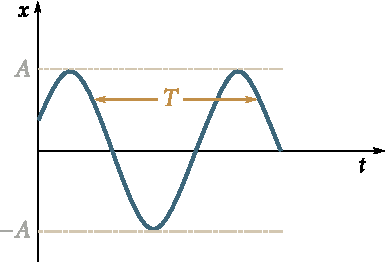
\includegraphics[scale=0.95]{figures/cap_07/fig_7_4.pdf}
		\caption[]{}
		\label{fig:7_4}
	\end{center}
	\vspace{-0.7cm}
\end{figure}

A graph of the harmonic oscillation, \ie, one of the function~\eqref{eq:7_55}, is shown in \fig{7_4}. The time $t$ is laid off along the horizontal axis, and the displacement $x$ along the vertical one. Since a cosine varies from $-1$ to $1$, then the values of $x$ range from $-A$ to $A$.

The maximum deviation of a system from its equilibrium position is called the \textbf{amplitude} of oscillation. The amplitude $A$ is a constant positive quantity. Its value is determined by the magnitude of the initial deviation or push that brought the system out of the equilibrium position.

The cosine argument ($\omega_0 t+\alpha$) is called the \textbf{phase} of oscillation. The constant $\alpha$ is the value of the phase at the moment $t=0$ and is called the \textbf{initial phase} of oscillation. The constant $\alpha$ will change when the moment from which we begin to measure the time is changed. Hence, the value of the initial phase is determined by when we begin to measure the time. Since the value of $x$ does not change when a whole number of $2\pi$'s is added to or subtracted from the phase, we can always ensure that the initial phase will be less than $\pi$ in magnitude. This is why only values of $\alpha$ within the limits from $-\pi$ to $+\pi$ are usually considered.

Since a cosine is a periodic function with the period $2\pi$, different states\footnote{We remind our reader that the state of a mechanical system is characterized by the values of the coordinates and the velocities of the bodies forming the system.} of a system performing harmonic oscillations repeat during the time interval $T$ in which the phase of oscillation receives an increment equal to $2\pi$ (\fig{7_4}). The interval $T$ is called the \textbf{period} of oscillation. It can be found from the condition $|\omega_0(t+T)+\alpha|=|\omega_0 t+\alpha|+2\pi$, whence
\begin{equation}\label{eq:7_56}
	T = \frac{2\pi}{\omega_0}.
\end{equation}

The number of oscillations in unit time is called the \textbf{frequency} of oscillation $\nu$. It is quite evident that the frequency $\nu$ is related to the duration of one oscillation $T$ by the expression
\begin{equation}\label{eq:7_57}
	\nu = \frac{1}{T}.
\end{equation}

\noindent
The unit of frequency is the frequency of oscillations whose period is \SI{1}{\second}. This unit is called the hertz (\si{\hertz}). A frequency of \SI{e3}{\hertz} is called a kilohertz (\si{\kilo\hertz}), and of \SI{e6}{\hertz} a megahertz (\si{\mega\hertz}).

It follows from \eqn{7_56} that
\begin{equation}\label{eq:7_58}
	\omega_0 = \frac{2\pi}{T}.
\end{equation}

\noindent
Thus, $\omega_0$ is the number of oscillations in $2\pi$ seconds. The quantity $\omega_0$ is called the \textbf{circular} or \textbf{cyclic} frequency. It is related to the conventional frequency $\nu$ by the expression
\begin{equation}\label{eq:7_59}
	\omega_0 = 2\pi\nu.
\end{equation}

Time differentiation of \eqn{7_55} yields an expression for the velocity:
\begin{equation}\label{eq:7_60}
	v = \dot{x} = -A\omega_0\sin(\omega_0 t + \alpha) = A\omega_0\cos\left(\omega_0 t + \alpha + \frac{\pi}{2}\right).
\end{equation}

\noindent
Examination of \eqn{7_60} shows that the velocity also changes according to a harmonic law, the amplitude of the velocity being $A\omega_0$. It follows from a comparison of Eqs.~\eqref{eq:7_55} and~\eqref{eq:7_60} that the phase of the velocity is in advance of that of the displacement
by $\pi/2$.

Time differentiation of \eqn{7_60} yields an expression for the acceleration:
\begin{equation}\label{eq:7_61}
	a = \ddot{x} = -A\omega_0^2\cos(\omega_0 t + \alpha) = A\omega_0^2\cos(\omega_0 t + \alpha + \pi).
\end{equation}

\noindent
It can be seen from \eqn{7_61} that the acceleration and the displacement are opposite in phase. This signifies that when the displacement reaches its maximum positive value, the acceleration reaches its maximum negative value, and vice versa.

Figure~\ref{fig:7_5} compares graphs for the displacement, velocity, and acceleration.

\begin{figure}[t]
	\begin{center}
		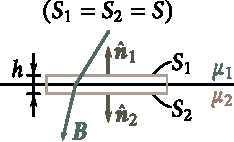
\includegraphics[scale=0.95]{figures/cap_07/fig_7_5.pdf}
		\caption[]{}
		\label{fig:7_5}
	\end{center}
	\vspace{-1.0cm}
\end{figure}

A particular oscillation is characterized by definite values of the amplitude $A$ and the initial phase $\alpha$. The values of these quantities for a given oscillation can be determined from the initial conditions, \ie, from the values of the deviation $x_0$ and the velocity $v_0$ at the initial moment. Indeed, assuming in Eqs.~\eqref{eq:7_55} and~\eqref{eq:7_60} that $t=0$, we get two equations:
\begin{equation*}
	x_0 = A\cos\alpha,\quad v_0 = -A\omega_0\sin\alpha
\end{equation*}

\noindent
from which we find that
\begin{align}
	A &= \left(x_0^2 + \frac{v_0^2}{\omega_0^2}\right)^{1/2}, \label{eq:7_62}\\
	\tan\alpha &= -\frac{v_0}{x_0\omega_0}.\label{eq:7_63}
\end{align}

\noindent
Equation~\eqref{eq:7_63} is satisfied by two values of $\alpha$ within the interval from $-\pi$ to $+\pi$. That value must be taken which gives the correct signs of cosine and sine.

A quasi-elastic force is conservative. Therefore, the total energy of a harmonic oscillation must remain constant. In the course of oscillations, kinetic energy transforms into potential energy, and vice versa. At the moments of maximum deviation from the equilibrium position, the total energy $E$ consists only of potential energy, which reaches its maximum value $E_{\text{p,max}}$:
\begin{equation}\label{eq:7_64}
	E = E_{\text{p,max}} = \frac{kA^2}{2}.
\end{equation}

\noindent
When the system passes through its equilibrium position, the total energy consists only of kinetic energy, which at these moments reaches its maximum value $E_{\text{k,max}}$:
\vspace{-12pt}
\begin{equation}\label{eq:7_65}
	E = E_{\text{k,max}} = \frac{mv_{\text{max}}^2}{2} = \frac{mA^2\omega_0^2}{2}
\end{equation}

\noindent
(it was shown above that the velocity amplitude is $A\omega_0$). Equations~\eqref{eq:7_64} and~\eqref{eq:7_65} equal each other because by \eqn{7_6} we have $m\omega_0^2=k$.

Let us see how the kinetic and potential energies of harmonic oscillations change with time. The kinetic energy is [see \eqn{7_60} for $\dot{x}$]
\begin{equation}\label{eq:7_66}
	E_{\text{k}} = \frac{m\dot{x}^2}{2} = \frac{mA^2\omega_0^2}{2}\sin^2(\omega_0 t + \alpha).
\end{equation}

\noindent
The potential energy is expressed by the equation
\begin{equation}\label{eq:7_67}
	E_{\text{p}} = \frac{kx^2}{2} = \frac{kA^2}{2}\cos^2(\omega_0 t + \alpha).
\end{equation}

\noindent
Adding Eqs.~\eqref{eq:7_66} and~\eqref{eq:7_67} and bearing in mind that $m\omega_0^2=k$, we get a formula for the total energy:
\begin{equation}\label{eq:7_68}
	E = E_{\text{k}} + E_{\text{p}}= \frac{kA^2}{2} = \frac{mA^2\omega_0^2}{2}
\end{equation}

\noindent
[compare with Eqs.~\eqref{eq:7_64} and~\eqref{eq:7_65}]. Thus, the total energy of a harmonic oscillation is indeed constant.

\begin{figure}[t]
	\begin{center}
		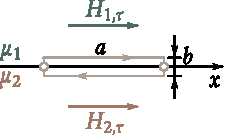
\includegraphics[scale=0.95]{figures/cap_07/fig_7_6.pdf}
		\caption[]{}
		\label{fig:7_6}
	\end{center}
	\vspace{-0.85cm}
\end{figure}

Using formulas of trigonometry, we can write the expressions for $E_{\text{k}}$ and $E_{\text{p}}$ as follows:
\begin{align}
	E_{\text{k}} &= E\sin^2(\omega_0 t + \alpha) = E \left\{\frac{1}{2} - \frac{1}{2}\cos[2(\omega_0 t + \alpha)]\right\}\label{eq:7_69}\\
	E_{\text{p}} &= E\cos^2(\omega_0 t + \alpha) = E \left\{\frac{1}{2} + \frac{1}{2}\cos[2(\omega_0 t + \alpha)]\right\}\label{eq:7_70}
\end{align}

\noindent
where $E$ is the total energy of the system. A glance at these equations shows that $E_{\text{k}}$ and $E_{\text{p}}$ change with a frequency of $2\omega_0$, \ie, with a frequency twice that of the harmonic oscillations. Figure~\ref{fig:7_6} compares graphs for $x$, $E_{\text{k}}$ and $E_{\text{p}}$.



It is known that the mean value of sine square and of cosine square equals one-half. Hence, the mean value of $E_{\text{k}}$ coincides with that of $E_{\text{p}}$ and equals $E/2$.

\section{The Pendulum}\label{sec:7_6}

Physicists understand a pendulum to be a rigid body performing oscillations about a fixed point or axis under the acting of the force of gravity.

A mathematical or simple pendulum is defined as an idealized system consisting of a weightless and unstretchable string on which a mass concentrated at one point is suspended. A sufficiently close approximation to a simple pendulum is a small heavy sphere suspended on a long thin thread.

\begin{figure}[t]
	\begin{center}
		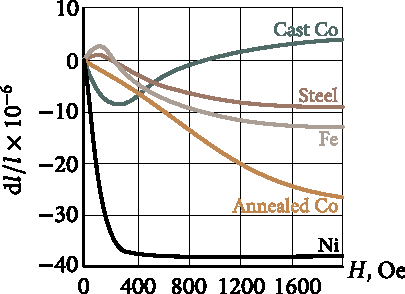
\includegraphics[scale=0.95]{figures/cap_07/fig_7_7.pdf}
		\caption[]{}
		\label{fig:7_7}
	\end{center}
	\vspace{-0.7cm}
\end{figure}

We shall characterize the deviation of a pendulum from its equilibrium position by the angle $\varphi$ made by the thread with a vertical line (\fig{7_7}). Deviation of a pendulum from its equilibrium position is attended by the appearance of a rotational moment (torque) $M$ whose magnitude is $mgl\sin\varphi$ (here $m$ is the mass and $l$ is the length of the pendulum). Its direction is such that it tends to return the pendulum to its equilibrium position, and is similar in this respect to a quasi-elastic force. Therefore, opposite signs must be assigned to the moment $M$ and the angular displacement $\varphi$\footnote{Considering $\varphi$ as a vector related to the direction of rotation by the right-hand screw rule (this is permissible at small values of $\varphi$), the opposite signs of	$M$ and $\varphi$ can be explained by the fact that the vectors $\vec{M}$ and $\vec{\varphi}$ have opposite	directions (\fig{7_7}).}, as is done to the displacement and the quasi-elastic force. Hence, the expression for the rotational moment has the form
\begin{equation}\label{eq:7_71}
	M = -mgl\sin\varphi.
\end{equation}

Let us write an equation for the dynamics of rotation of a pendulum. Denoting the angular acceleration by $\ddot{\varphi}$ and taking into account that the moment of inertia of a pendulum is $ml^2$ we get
\begin{equation*}
	ml^2\ddot{\varphi} = -mgl\sin\varphi.
\end{equation*}

\noindent
This equation can be transformed as follows:
\begin{equation}\label{eq:7_72}
	\ddot{\varphi} + \frac{g}{l}\sin\varphi = 0.
\end{equation}

Let us consider only small-amplitude oscillations. We can thus assume that $\sin\varphi\approx\varphi$. Introducing, in addition, the notation
\begin{equation}\label{eq:7_73}
	\frac{g}{l} = \omega_0^2
\end{equation}

\noindent
we arrive at the equation
\begin{equation}\label{eq:7_74}
	\ddot{\varphi} + \omega_0^2\varphi = 0
\end{equation}

\noindent
similar to \eqn{7_7}. Its solution has the form
\begin{equation}\label{eq:7_75}
	\varphi = A\cos(\omega_0 t + \alpha).
\end{equation}

\noindent
Consequently, in small-amplitude oscillations, the angular displacement of a simple pendulum changes with time according to a harmonic law.

Equation~\eqref{eq:7_73} shows that the frequency of oscillations of a simple pendulum depends only on its length and on the acceleration of the force of gravity and does not depend on the mass of the pendulum. Equation~\eqref{eq:7_56} after~\eqref{eq:7_73} is introduced into it gives the expression for the period of oscillations of a simple pendulum known from school days:
\begin{equation}\label{eq:7_76}
	T = 2\pi\left(\frac{l}{g}\right)^{1/2}.
\end{equation}

By solving \eqn{7_72}, we can obtain the following formula for the period of oscillations:
\begin{equation}\label{eq:7_77}
	T = 2\pi\left(\frac{l}{g}\right)^{1/2}\left\{1 + \left(\frac{1}{2}\right)^2 \sin^2\frac{A}{2} + \left(\frac{1}{2}\times\frac{3}{4}\right)^2\sin^4\frac{A}{2} + \ldots\right\}.
\end{equation}

\noindent
where $A$ is the amplitude of the oscillations, \ie, the greatest angle through which a pendulum deflects from its equilibrium position.

\begin{figure}[t]
	\begin{center}
		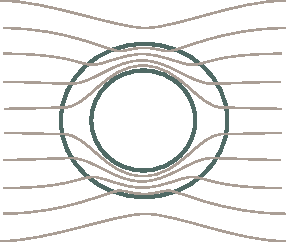
\includegraphics[scale=0.9]{figures/cap_07/fig_7_8.pdf}
		\caption[]{}
		\label{fig:7_8}
	\end{center}
	\vspace{-0.8cm}
\end{figure}

If an oscillating body cannot be treated as a point particle, the pendulum is called a physical one. When the pendulum deviates from its equilibrium position by the angle $\varphi$, a rotational moment (torque) appears that tends to return the pendulum to its equilibrium position. This moment is
\begin{equation}\label{eq:7_78}
	M = -mgl\sin\varphi
\end{equation}

\noindent
where $m$ is the mass of the pendulum and $l$ is the distance between the suspension point $0$ and the centre of mass C of the pendulum (\fig{7_8}). The minus sign has the same meaning as in \eqn{7_71}.

Denoting the moment of inertia of a pendulum relative to the axis passing through the point of suspension by the symbol $I$, we can write:
\begin{equation}\label{eq:7_79}
	I\ddot{\varphi} = -mgl\sin\varphi.
\end{equation}

\noindent
For small-amplitude oscillations, \eqn{7_79} transforms into \eqn{7_74} that we already know:
\begin{equation*}
	\ddot{\varphi} +\omega_0^2\varphi = 0.
\end{equation*}

\noindent
Here $\omega_0^2$ stands for the following quantity:
\begin{equation}\label{eq:7_80}
	\omega_0^2 = \frac{mgl}{I}.
\end{equation}

It follows from Eqs.~\eqref{eq:7_74} and~\eqref{eq:7_80} that with small displacements from the equilibrium position, a physical pendulum performs harmonic oscillations whose frequency depends on the mass of the pendulum, the moment of inertia of the pendulum relative to the axis of rotation, and the distance between the latter and the centre of mass of the pendulum. According to \eqn{7_80}, the period of oscillation of a physical pendulum is determined by the expression
\begin{equation}\label{eq:7_81}
	T = 2\pi\left(\frac{I}{mgl}\right)^{1/2}.
\end{equation}

\noindent
A comparison of Eqs.~\eqref{eq:7_76} and~\eqref{eq:7_81} shows that a mathematical pendulum of length
\vspace{-12pt}
\begin{equation}\label{eq:7_82}
	l_{\text{r}} = \frac{I}{ml}
\end{equation}

\noindent
will have the same period of oscillations as the given physical pendulum. The quantity~\eqref{eq:7_82} is called the \textbf{reduced length} of the physical pendulum. Thus, the reduced length of a physical pendulum is the length of a simple pendulum whose period of oscillations coincides with that of the given physical pendulum.

The point on the straight line joining the point of suspension to the centre of mass at a distance of the reduced length from the axis of rotation is called the \textbf{centre of oscillation} of the physical pendulum (see point $0'$ in \fig{7_8}). It can be shown (we invite our reader to do this as an exercise) that when a pendulum is suspended by its centre of oscillation $0'$, its reduced length and, consequently, its period of oscillations will be the same as initially. Hence, the point of suspension and the centre of oscillation are interchangeable: when the point of suspension is transferred to the centre of oscillation, the previous point of suspension becomes the new centre of oscillation. This property underlies the determination of the acceleration of free fall with the aid of the so-called reversible pendulum. The latter has two parallel knife edges fastened near its ends by which it can be suspended in turn. Heavy weights can be moved along the pendulum and be fastened to it. The weights are adjusted to ensure the pendulum having the same period of oscillations when suspended by any of the knife edges. In this case, the distance between the knife edges will be $l_{\text{r}}$. By measuring the period of oscillations of the pendulum and knowing $l$, we can find the acceleration of free fall $g$ by the equation
\begin{equation*}
	T = 2\pi\left(\frac{l_{\text{r}}}{g}\right)^{1/2}.
\end{equation*}

\section{Vector Diagram}\label{sec:7_7}

The solution of a number of problems, particularly the addition of several oscillations of the same direction (or, which is the same the addition of several harmonic functions) is considerably facilitated and becomes clear if we depict oscillations graphically in the form of vectors in a plane. The result obtained is called a \textbf{vector diagram}.

Let us take an axis which we shall denote by the symbol $x$ (\fig{7_9}). From point $0$ on the axis we shall lay off a vector of length $A$ making the angle $\alpha$ with the axis. If we rotate this vector with the angular velocity $\omega_0$, then the projection of the end of the vector will move along the $x$-axis within the limits from $-A$ to $+A$. The coordinate of this projection will change with time according to the law
\begin{equation*}
	x = A\cos(\omega_0 t + \alpha).
\end{equation*}

\noindent
Consequently, the projection of the tip of the vector onto the axis will perform a harmonic oscillation with an amplitude equal to the length of the vector, an angular frequency equal to the angular velocity of the vector, and an initial phase equal to the angle formed by the vector with the axis at the initial moment.

It follows from the above that a harmonic oscillation can be given with the aid of a vector whose length equals the amplitude of the oscillation, while the direction of the vector makes an angle with the $x$-axis that equals the initial phase of the oscillation.

\begin{figure}[t]
	\begin{center}
		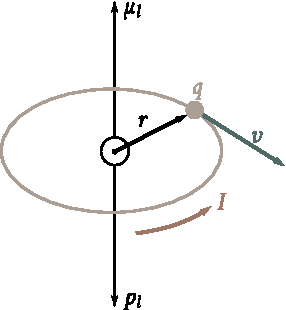
\includegraphics[scale=0.95]{figures/cap_07/fig_7_9.pdf}
		\caption[]{}
		\label{fig:7_9}
	\end{center}
	\vspace{-0.8cm}
\end{figure}

Let us consider the addition of two harmonic oscillations of the same direction and the same frequency. The displacement $x$ of the oscillating body will be the sum of the displacements $x_1$ and $x_2$, which can be written as follows:
\begin{equation}\label{eq:7_83}
	x_1 = A_1\cos(\omega_0 t + \alpha_1),\quad x_2 = A_2\cos(\omega_0 t + \alpha_2).
\end{equation}

\noindent
Let us represent both oscillations with the aid of the vectors $\vec{A}_1$ and $\vec{A}_2$ (\fig{7_10}). We shall construct the resultant vector $\vec{A}$ according to the rules of vector addition. It is easy to see that the projection of this vector onto the $x$-axis equals the sum of the projections of the vectors being added:
\begin{equation*}
	x = x_1 + x_2.
\end{equation*}

\noindent
Consequently, the vector $\vec{A}$ is the resultant oscillation. This vector rotates with the same angular velocity as the vectors $\vec{A}_1$ and $\vec{A}_2$ so that the resultant motion will be a harmonic oscillation with the frequency $\omega_0$, amplitude $A$, and the initial phase $\alpha$. It can be seen from the construction that
\begin{align}
	A^2 &= A_1^2 + A_2^2 - 2A_1A_2\cos[\pi-(\alpha_2-\alpha_1)] \nonumber\\
	&= A_1^2 + A_2^2 - 2A_1A_2\cos(\alpha_2-\alpha_1), \label{eq:7_84}\\
	\tan\alpha &= \frac{A_1\sin\alpha_1 + A_2\sin\alpha_2}{A_1\cos\alpha_1 + A_2\cos\alpha_2}.\label{eq:7_85}
\end{align}

Thus, the representation of harmonic oscillations by means of vectors makes it possible to reduce the addition of several oscillations to the operation of vector addition. This procedure is especially useful in optics, for example, where the light oscillations at a point are determined as the result of the superposition of many oscillations arriving at the given point from different sections of a wavefront. 

\begin{figure}[t]
	\begin{center}
		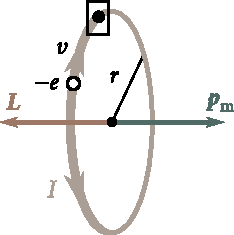
\includegraphics[scale=0.95]{figures/cap_07/fig_7_10.pdf}
		\caption[]{}
		\label{fig:7_10}
	\end{center}
	\vspace{-0.8cm}
\end{figure}

Equations~\eqref{eq:7_84} and~\eqref{eq:7_85} can naturally be obtained by summation of Eqs.~\eqref{eq:7_83} and the corresponding trigonometric transformations. But the way we have used to obtain these equations is distinguished by its great simplicity and clarity.

Let us analyse \eqn{7_84} for the amplitude. If the difference between the phases of both oscillations $\alpha_2-\alpha_1$ vanishes, the amplitude of the resulting oscillation equals the sum of $A_1$ and $A_ 2$. If the phase difference $\alpha_2-\alpha_1$ equals $+\pi$ or $-\pi$, \ie, both oscillations are in counterphase, then the amplitude of the resulting oscillation equals $|A_1-A_2|$.

If the frequencies of the oscillations $x_1$ and $x_2$ are not the same, the vectors $\vec{A}_1$ and $\vec{A}_2$ will rotate with different velocities. In this case, the resultant vector $\vec{A}$ pulsates in magnitude and rotates with a varying velocity. Consequently, the resultant motion in this case will be a complex oscillating process instead of a harmonic oscillation.

\section{Beats}\label{sec:7_8}

Of special interest is the case when two harmonic oscillations of the same direction being added differ only slightly in frequency. We shall now show that the resultant motion in these conditions can be considered as a harmonic oscillation with a pulsating amplitude. Such oscillations are called \textbf{beats}.

Let $\omega$ stand for the frequency of one of the oscillations and $\omega+\Delta\omega$ for that of the second one. According to our conditions, $\Delta\omega\ll\omega$. We shall assume that the amplitudes of both oscillations are the same and equal $A$. To avoid unnecessary complications in our formulas, we shall consider that the initial phases of both oscillations equal zero. The equations of the oscillations will thus become
\begin{equation*}
	x_1 = A\cos\omega t,\quad x_2 = A\cos(\omega+\Delta\omega) t.
\end{equation*}

\noindent
By summing these expressions and using the trigonometric formula for the sum of cosines, we get
\begin{equation}\label{eq:7_86}
	x = x_1 + x_2 = \left[ 2A \cos\left(\frac{\Delta\omega}{2}t\right)\right] \cos\omega t
\end{equation}

\noindent
(in the second multiplier we disregard the term $\Delta\omega/2$ in comparison with $\omega$). A graph of the function~\eqref{eq:7_86} is shown in \fig{7_11}a. The graph has been plotted for $\omega/\Delta\omega=10$.

\begin{figure}[t]
	\begin{minipage}[t]{0.5\linewidth}
		\begin{center}
			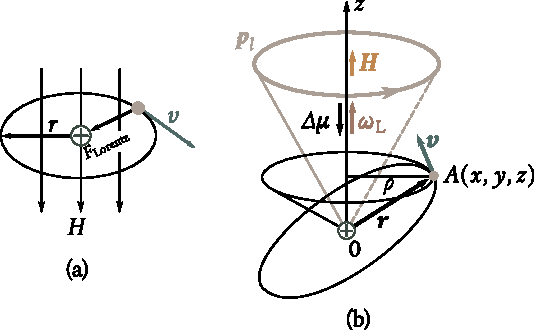
\includegraphics[scale=1.0]{figures/cap_07/fig_7_11.pdf}
			\caption[]{}
			\label{fig:7_11}
		\end{center}
	\end{minipage}
	\hspace{-0.0cm}
	\begin{minipage}[t]{0.5\linewidth}
		\begin{center}
			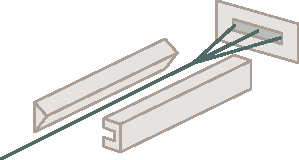
\includegraphics[scale=0.85]{figures/cap_07/fig_7_12.pdf}
			\caption[]{}
			\label{fig:7_12}
		\end{center}
	\end{minipage}
	\vspace{-0.6cm}
\end{figure}

The multiplier in parentheses in \eqn{7_86} changes much more slowly than the second multiplier. Owing to the condition $\Delta\omega\ll\omega$, the multiplier in parentheses does not virtually change during the time in which the multiplier $\cos\omega t$ performs several complete oscillations. This gives us the grounds to consider the oscillation~\eqref{eq:7_86} as a harmonic oscillation of frequency $\omega$ whose amplitude changes according to a periodic law. The multiplier in parentheses cannot be an expression of this law because it changes within the limits from $-2A$ to $+2A$ whereas the amplitude by definition is a positive quantity. A graph of the amplitude is shown in \fig{7_11}b. The analytic expression of the amplitude obviously has the form
\begin{equation}\label{eq:7_87}
	\text{amplitude} = \left|2A\cos\left(\frac{\Delta\omega}{2}t\right)\right|.
\end{equation}

The function~\eqref{eq:7_87} is a periodic function with a frequency double that of the expression inside the magnitude sign (see \fig{7_12} comparing graphs of the cosine and its magnitude), \ie, with a frequency of $\Delta\omega$. Thus, the frequency of pulsations of the amplitude---it is called the frequency of the beats---equals the difference between the frequencies of the oscillations being added.

We must note that the multiplier $2A\cos(\Delta\omega t/2)$ not only determines the amplitude, but also affects the phase of the oscillations. This is manifested, for example, in that the deflections corresponding to adjacent peaks of the amplitude have opposite signs (see points M$_1$ and M$_2$ in \fig{7_11}a).

\section{Addition of Mutually Perpendicular Oscillations}\label{sec:7_9}

Assume that a point particle can oscillate both along the $x$-axis and along the $y$-axis perpendicular to it. If we induce both oscillations, the particle will move along a certain, generally speaking, curved trajectory whose shape depends on the phase difference between the two oscillations.

Let us choose the beginning of counting time so that the initial phase of the first oscillation equals zero. The equations of the oscillations will therefore be written as follows:
\begin{equation}\label{eq:7_88}
	x = A\cos\omega t,\quad y = B\cos(\omega t + \alpha)
\end{equation}

\noindent
where $\alpha$ is the difference between the phases of the two oscillations.

Equations~\eqref{eq:7_88} describe the trajectory along which a body participating in both oscillations moves and are given in the parametric form. To obtain an equation of the trajectory in the conventional form, we must exclude the parameter $t$ from Eqs.~\eqref{eq:7_88}. It follows from the first of the Eqs.\eqref{eq:7_88} that
\begin{equation}\label{eq:7_89}
	\cos\omega t = \frac{x}{A}.
\end{equation}

\noindent
Hence,
\begin{equation}\label{eq:7_90}
	\sin\omega t = \left(1 - \frac{x^2}{A^2}\right)^{1/2}.
\end{equation}

\noindent
Now let us expand the cosine in the second of the Eqs.~\eqref{eq:7_88} according to the formula for the cosine of a sum, using instead of $\cos\omega t$ and $\sin\omega t$ their values from Eqs.~\eqref{eq:7_89} and~\eqref{eq:7_90}. As a result we get
\begin{equation*}
	\frac{y}{A} = \frac{x}{A}\cos\alpha - \sin\alpha \left(1 - \frac{x^2}{A^2}\right)^{1/2}.
\end{equation*}

\noindent
This equation after simple transformations can be given the form
\begin{equation}\label{eq:7_91}
	\frac{x^2}{A^2} + \frac{y^2}{B^2} - \frac{2xy}{AB} \cos\alpha = \sin^2\alpha.
\end{equation}

It is known from analytical geometry that \eqn{7_91} is the equation of an ellipse whose axes are oriented arbitrarily relative to the coordinate axes $x$ and $y$. The orientation of the ellipse and the dimensions of its semiaxes depend in a quite complicated way on the amplitudes $A$ and $B$ and the phase difference $\alpha$.

Let us study the shape of the trajectory in some particular cases.

\begin{enumerate}[1.]
	\item The phase difference a equals zero. In this case, \eqn{7_91} becomes
	\begin{equation*}
		\left(\frac{x}{A} - \frac{y}{B}\right)^{2} = 0
	\end{equation*}
	
	\noindent
	whence we get an equation of a straight line:
	\begin{equation}\label{eq:7_92}
		y = \frac{B}{A}x.
	\end{equation}
	
	\noindent
	The oscillating particle moves along this straight line, its distance from the origin of coordinates being $r=\sqrt{x^2+y^2}$. Introducing into this equation the expressions~\eqref{eq:7_88} for $x$ and $y$ and taking into account that $a=0$, we get the law of the change in $r$ with time:
	\begin{equation}\label{eq:7_93}
		r = \left(x^2 + y^2\right)^{1/2}\cos\omega t.
	\end{equation}
	
	\noindent
	It follows from \eqn{7_93} that the resultant motion is a harmonic oscillation along the straight line~\eqref{eq:7_92} with the frequency $\omega$ and the amplitude $\sqrt{A^2+B^2}$ (\fig{7_13}).
	
	\item The phase difference a equals $\pm\pi$. Equation~\eqref{eq:7_91} has the form
	\begin{equation*}
		\left(\frac{x}{A} + \frac{y}{B}\right)^{2} = 0
	\end{equation*}
	
	\noindent
	whence we find that the resultant motion is a harmonic oscillation along a straight line (\fig{7_14}):
	\begin{equation*}
		y = -\frac{B}{A}x.
	\end{equation*}
	
	\item When $\alpha=\pm\pi/2$, \eqn{7_91} becomes
	\begin{equation}\label{eq:7_94}
		\frac{x^2}{A^2} + \frac{y^2}{B^2} = 1
	\end{equation}

	\noindent
	\ie, it becomes the equation of an ellipse reduced to the coordinate axes, the semiaxes of the ellipse being equal to the corresponding amplitudes of the oscillations. When the amplitudes $A$ and $B$ are equal, the ellipse degenerates into a circle.
	
	The cases $\alpha=+\pi/2$ and $\alpha=-\pi/2$ differ in the direction of motion along the ellipse or circle. If $\alpha=+\pi/2$, Eqs.~\eqref{7_88} can be written as follows:
	\begin{equation}\label{eq:7_95}
		x = A\cos\omega t,\quad y = -B\sin\omega t.
	\end{equation}
	
	\noindent
	At the moment $t=0$, the body is at point $1$ (\fig{7_15}). At the following moments, the coordinate $x$ diminishes, while the coordinate $y$ becomes negative. Consequently, the motion is clockwise.
	
	When $\alpha=-\pi/2$, the equations of the oscillations become
	\begin{equation}\label{eq:7_96}
		x = A\cos\omega t,\quad y = B\sin\omega t.
	\end{equation}
	
	\noindent
	Hence we can conclude that the motion is counter-clockwise.
\end{enumerate}

\begin{figure}[t]
	\begin{minipage}[t]{0.5\linewidth}
		\begin{center}
			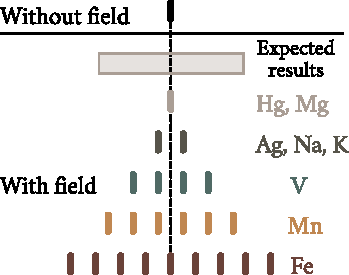
\includegraphics[scale=0.95]{figures/cap_07/fig_7_13.pdf}
			\caption[]{}
			\label{fig:7_13}
		\end{center}
	\end{minipage}
	\hspace{-0.0cm}
	\begin{minipage}[t]{0.5\linewidth}
		\begin{center}
			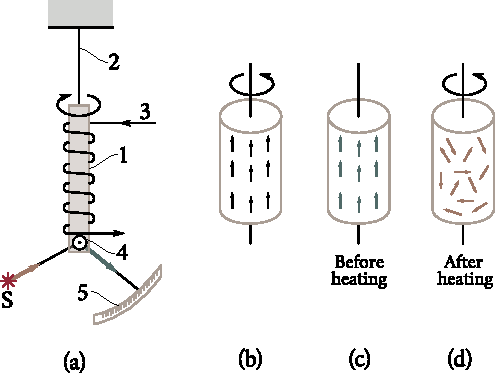
\includegraphics[scale=0.95]{figures/cap_07/fig_7_14.pdf}
			\caption[]{}
			\label{fig:7_14}
		\end{center}
	\end{minipage}
	\vspace{-0.6cm}
\end{figure}

\begin{figure}[t]
	\begin{minipage}[t]{0.5\linewidth}
		\begin{center}
			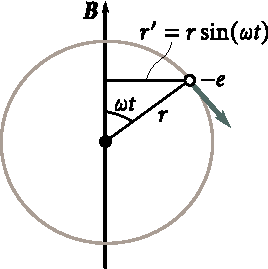
\includegraphics[scale=0.95]{figures/cap_07/fig_7_15.pdf}
			\caption[]{}
			\label{fig:7_15}
		\end{center}
	\end{minipage}
	\hspace{-0.0cm}
	\begin{minipage}[t]{0.5\linewidth}
		\begin{center}
			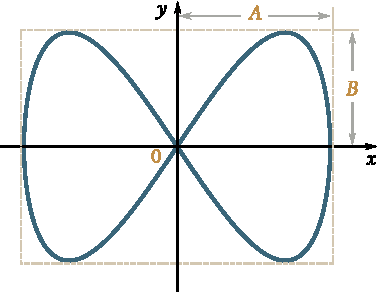
\includegraphics[scale=0.95]{figures/cap_07/fig_7_16.pdf}
			\caption[]{}
			\label{fig:7_16}
		\end{center}
	\end{minipage}
	\vspace{-0.6cm}
\end{figure}

It follows from the above that uniform motion along a circle of radius $R$ with the angular velocity $\omega$ can be represented as the sum of two mutually perpendicular oscillations:
\begin{equation}\label{eq:7_97}
	x = R\cos\omega t,\quad y = \pm R\sin\omega t
\end{equation}

\noindent
(the plus sign in the expression for $y$ corresponds to counter-clockwise motion, and the minus sign to clockwise motion).

When the frequencies of mutually perpendicular oscillations differ by a very small value $\Delta\omega$, they can be considered as oscillations of an identical frequency, but with a slowly changing phase difference. Indeed, the equations of the oscillations can be written as follows:
\begin{equation*}
	x = A\cos\omega t,\quad y = B\cos[\omega t + (\Delta\omega t + \alpha)]
\end{equation*}

\noindent
and the expression $\Delta\omega t + \alpha$ can be considered as the phase difference slowly changing with time according to a linear law.

The resultant motion in this case occurs along a slowly changing curve that will sequentially take on a shape corresponding to all the values of the phase difference from $-\pi$ to $+\pi$.

If the frequencies of mutually perpendicular oscillations are not identical, then the trajectory of the resultant motion has the shape of rather intricate curves called \textbf{Lissajous figures}. Figure~\ref{fig:7_16} shows one of the simple trajectories obtained at a frequency ratio of $1$:$2$ and a phase difference of $\pi/2$. The equations of the oscillations have the form
\begin{equation*}
	x = A\cos\omega t,\quad y = B\cos\left(\omega t + \frac{\pi}{2}\right).
\end{equation*}

\noindent
During the time the particle manages to move from one  extreme position to the other along the $x$-axis, it will be able to leave its zero position, reach one extreme position on the $y$-axis, then the other one, and return to its zero position.

With a frequency ratio of $1$:$2$ and a phase difference of zero, the trajectory degenerates into an open curve (\fig{7_17}) along which the particle moves to and fro.

\begin{figure}[t]
	\begin{minipage}[t]{0.5\linewidth}
		\begin{center}
			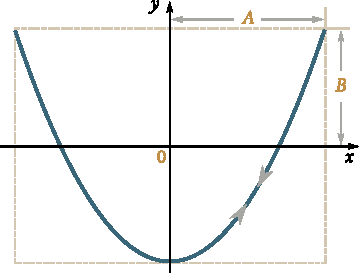
\includegraphics[scale=0.95]{figures/cap_07/fig_7_17.pdf}
			\caption[]{}
			\label{fig:7_17}
		\end{center}
	\end{minipage}
	\hspace{-0.05cm}
	\begin{minipage}[t]{0.5\linewidth}
		\begin{center}
			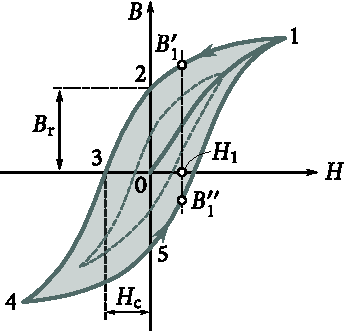
\includegraphics[scale=0.95]{figures/cap_07/fig_7_18.pdf}
			\caption[]{}
			\label{fig:7_18}
		\end{center}
	\end{minipage}
	\vspace{-0.6cm}
\end{figure}

The closer to unity is the rational fraction expressing the ratio of the frequencies of the oscillations, the more intricate is the Lissajous figure. Figure~\ref{fig:7_18} shows as an example a curve for the frequency ratio of $3$:$4$ and the phase difference $\pi/2$.

\section{Damped Oscillations}\label{sec:7_10}

Damped oscillations are described by \eqn{7_11}:
\begin{equation*}
	\ddot{x} + 2\beta\dot{x} + \omega_0^2 x = 0
\end{equation*}

\noindent
where, by Eqs.~\eqref{eq:7_10} and~\eqref{eq:7_6},
\begin{equation*}
	2\beta = \frac{r}{m},\quad \omega_0^2 = \frac{k}{m}.
\end{equation*}

\noindent
Here $r$ is the resistance coefficient, \ie, the coefficient of proportionality between the velocity $x$ and the force of resistance, and $k$ is the quasi-elastic force coefficient. We must note that $\omega_0$ is the frequency with which free oscillations would take place in the absence of resistance of the medium (when $r=0$). This frequency is called the \textbf{natural frequency} of the system.

Introduction of the function $x=e^{\lambda t}$ into \eqn{7_11} leads to the characteristic equation
\begin{equation}\label{eq:7_98}
	\lambda^2 + 2\beta\lambda + \omega_0^2 = 0.
\end{equation}

\noindent
The roots of this equation are
\begin{equation}\label{eq:7_99}
	\lambda_1 = -\beta + \left(\beta^2 - \omega_0^2\right)^{1/2},\quad \lambda_2 = -\beta - \left(\beta^2 - \omega_0^2\right)^{1/2}.
\end{equation}

When the damping is not too great (at $\beta<\omega_0$) the radicand will be negative. Let us write it in the form $(i\omega)^2$, where $\omega$ is a real quantity equal to
\begin{equation}\label{eq:7_100}
	\omega = \left(\beta^2 - \omega_0^2\right)^{1/2}.
\end{equation}

\noindent
Here, the roots of the characteristic equation will be as follows:
\begin{equation}\label{eq:7_101}
	\lambda_1 = -\beta + i\omega,\quad \lambda_2 = -\beta - i\omega.
\end{equation}

By \eqn{7_38}, the general solution of \eqn{7_11} will be the function
\begin{equation*}
	x = C_1e^{(-\beta + i\omega)t} + C_2e^{(-\beta - i\omega)t} = e^{\beta t} \left(C_1e^{i\omega t} + C_2e^{-i\omega t}\right).
\end{equation*}

\noindent
The expression in parentheses is similar to \eqn{7_51}. It can therefore be written in a form similar to \eqn{7_55}. Thus, when damping is not too great, the general solution of \eqn{7_11} has the form
\begin{equation}\label{eq:7_102}
	x = A_0 e^{\beta t} \cos(\omega t + \alpha).
\end{equation}

\noindent
Here $A_0$ and $\alpha$ are arbitrary constants, and $\omega$ is a quantity determined by \eqn{7_100}. Figure~\ref{fig:7_19} gives a graph of the function~\eqref{eq:7_102}. The dash lines show the limits confining the displacement $x$ of the oscillating particle.

In accordance with the kind of the function~\eqref{eq:7_102}, the motion of the system can be considered as a harmonic oscillation of frequency $\omega$ with an amplitude varying according to the law $A(t)=A_0e^{-\beta t}$. The upper dash curve in \fig{7_19} depicts the function $A(t)$, the quantity $A_0$ being the amplitude at the initial moment of time. The initial displacement $x_0$, apart from $A_0$, also depends on the initial phase $\alpha$: $x_0=A_0\cos\alpha$.

\begin{figure}[t]
	\begin{center}
		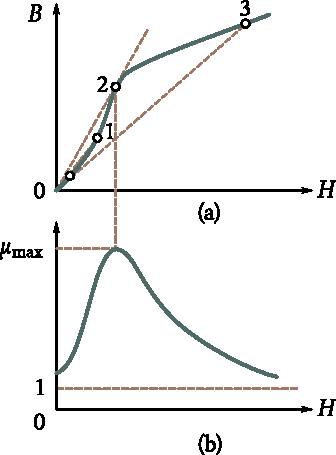
\includegraphics[scale=1.0]{figures/cap_07/fig_7_19.pdf}
		\caption[]{}
		\label{fig:7_19}
	\end{center}
	\vspace{-0.8cm}
\end{figure}

The rate of damping of oscillations is determined by the quantity $\beta=r/(2m)$ defined as the \textbf{damping factor}. Let us find the time $\tau$ during which the amplitude diminishes $e$ times. By definition, $e^{-\beta\tau}=e^{-1}$, whence $\beta\tau=1$. Consequently, the damping factor is the reciprocal of the time interval during which the amplitude diminishes $e$ times.

According to \eqn{7_56}, the period of damped oscillations is
\begin{equation}\label{eq:7_103}
	T = \frac{2\pi}{\left(\omega_0^2 - \beta^2\right)^{1/2}}.
\end{equation}

\noindent
When the resistance of the medium is insignificant, the period of oscillations virtually equals $T_0=2\pi/\omega_0$. The period of oscillations grows with an increasing damping factor.

The following maximum displacements to either side (for example $A', A'', A'''$, etc. in \fig{7_19}) form a geometrical progression. Indeed, if $A'=A_0e^{-\beta t}$, then $A''=A_0e^{-\beta(t+T)}=A'e^{-\beta T}$, $A'''=A_0e^{[-\beta(t+2T)]}=A''e^{-\beta T}$, etc. In general, the ratio of the values of the amplitudes corresponding to moments of time differing by a period is
\begin{equation*}
	\frac{A(t)}{A(t+T)} = e^{\beta T}.
\end{equation*}

\noindent
This ratio is called the \textbf{damping decrement}, and its logarithm is called the \textbf{logarithmic decrement}:
\begin{equation}\label{eq:7_104}
	\lambda = \ln\left[\frac{A(t)}{A(t+T)}\right] = \beta T
\end{equation}

\noindent
[do not confuse with the constant $\lambda$ in Eqs.~\eqref{eq:7_98} and~\eqref{eq:7_101}].

To characterize an oscillatory system, the logarithmic decrement $\lambda$ is usually used. Expressing $\beta$ through $\lambda$ and $T$ in accordance with \eqn{7_104}, we can write the law of diminishing of the amplitude with time in the form
\begin{equation}\label{eq:7_105}
	A = A_0\exp\left(-\frac{\lambda}{T}\,t\right).
\end{equation}

\noindent
In the interval during which the amplitude diminishes $e$ times, the system manages to complete $N_e=\tau/T$ oscillations. We find from the condition $\exp(-\lambda t/T)=\exp(-1)$ that $\lambda t/T=1$. Hence the logarithmic decrement is the reciprocal of the number of oscillations completed during the interval in which the amplitude diminishes $e$ times.

An oscillatory system is often also characterized by the quantity
\begin{equation}\label{eq:7_106}
	Q = \frac{\pi}{\lambda} = \pi N_e
\end{equation}

\noindent
called the \textbf{quality}, or simply the $Q$, of the system. As can be seen from its definition, the quality is proportional to the number of oscillations $N_e$ performed by the system in the interval $\tau$ during which the amplitude of the oscillations diminishes $e$ times.

We established in Sec.~\ref{sec:7_5} that the total energy of an oscillating system is proportional to the square of the amplitude [see \eqn{7_68}]. Accordingly, the energy of the system in damped oscillations diminishes with time according to the law
\begin{equation}\label{eq:7_107}
	E = E_0 e^{-2\beta t}
\end{equation}

\noindent
($E_0$ is the value of the energy at $t=0$). Time differentiation of this expression gives the rate of growth of the system's energy:
\begin{equation*}
	\diff{E}{t} = -2\beta E_0 e^{-2\beta t} = -2\beta E.
\end{equation*}

\noindent
By reversing the signs, we find the rate of diminishing of the energy:
\begin{equation}\label{eq:7_108}
	-\diff{E}{t} = 2\beta E.
\end{equation}

\noindent
If the energy changes only slightly during the time equal to a period of oscillations, the reduction of the energy during a period can be found by multiplying \eqn{7_108} by $T$:
\begin{equation*}
	-\Delta E = 2\beta T E
\end{equation*}

\noindent
(we remind our reader that $\Delta E$ stands for the increment, and $-\Delta E$ for the decrement of the energy). Finally, taking into consideration Eqs.~\eqref{eq:7_104} and~\eqref{eq:7_106}, we arrive at the relation
\begin{equation}\label{eq:7_109}
	\frac{E}{(-\Delta E)} = \frac{Q}{2\pi}
\end{equation}

\noindent
from which it follows that upon slight damping of oscillations, the quality with an accuracy up to the factor $2\pi$ equals the ratio of the energy stored in the system at a given moment to the decrement of this energy during one period of oscillations.

\begin{figure}[t]
	\begin{center}
		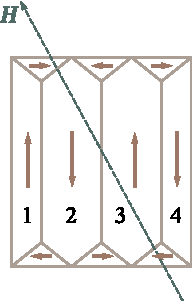
\includegraphics[scale=0.95]{figures/cap_07/fig_7_20.pdf}
		\caption[]{}
		\label{fig:7_20}
	\end{center}
	\vspace{-0.8cm}
\end{figure}

It follows from \eqn{7_103} that a growth in the damping factor is attended by an increase in the period of oscillations. At $\beta=\omega_0$, the period of oscillations becomes infinite, \ie, the motion stops being periodic. 

At $\beta>\omega_0$, the roots of the characteristic equation become real [see \eqn{7_99}], and the solution of the differential equation~\eqref{eq:7_11} is equal to the sum of two exponents:
\begin{equation*}
	x = C_1e^{-\lambda_1 t} + C_2e^{-\lambda_2 t}.
\end{equation*}

\noindent
Here $C_1$ and $C_2$ are real constants whose values depend on the initial conditions (on $x_0$ and $v_0=\dot{x}_0$). The motion is therefore aperiodic---a system displaced from its equilibrium position returns to it without performing oscillations. Figure~\ref{fig:7_20} shows two possible ways for a system to return to its equilibrium position in aperiodic motion. How the system arrives at its equilibrium position depends on the initial conditions. The motion depicted by curve $2$ is obtained when the system begins to move from the position characterized by the displacement $x_0$ to its equilibrium position with the initial velocity $v_0$ determined by the condition
\begin{equation}\label{eq:7_110}
	|v_0| > |x_0|\left[\beta + \left(\beta^2 + \omega_0^2\right)^{1/2}\right].
\end{equation}

\noindent
This condition will be obeyed when a system brought out of its equilibrium position is given a sufficiently strong impetus toward it. If after displacing a system from its equilibrium position we release it without an impetus (\ie, with $v_0=0$) or impart to it an impetus of insufficient force [such that $v_0$ is less than the value determined by the condition~\eqref{eq:7_110}], the motion will occur according to curve $1$ in \fig{7_20}.

\section{Auto-Oscillations}\label{sec:7_11}

The energy of a system in damped oscillations is used to overcome the resistance of the medium. If this decrease of energy is replenished, the oscillations will become undamped. The energy of a system can be replenished at the expense of impetuses from outside, but they must be imparted to the system in step with its oscillations, otherwise they may weaken the latter and even stop them. An oscillating system can be made to control the external action itself, ensuring agreement between the impetuses imparted to it and its motion. Such a system is called an \textbf{auto-oscillating} one, and the undamped oscillations it performs are called \textbf{auto-oscillations}.

\begin{figure}[t]
	\begin{center}
		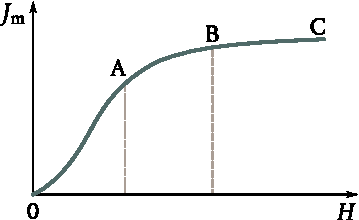
\includegraphics[scale=0.95]{figures/cap_07/fig_7_21.pdf}
		\caption[]{}
		\label{fig:7_21}
	\end{center}
	\vspace{-0.8cm}
\end{figure}

Let us consider a clock mechanism as an example of an auto-oscillatory system. The clock pendulum is fitted onto the same axis as a bent lever-the anchor (\fig{7_11}). The ends of the anchor carry projections of a special shape called pallets. The toothed escape wheel is acted upon by a chain with a weight or a wound up spring that tends to turn it clockwise. During the major part of the time, however, one of the wheel's teeth bears against the side face of a pallet, the latter sliding along the tooth's surface when the pendulum oscillates. Only when the pendulum is near its middle position do the pallets stop being in the way of the teeth, and the escape wheel turns, pushing the anchor by means of a tooth whose tip slides along the chamfered end of a pallet. During a complete cycle of pendulum oscillations (during a period), the escape wheel turns through two teeth, and each of the pallets receives a push. These pushes, performed at the expense of the energy of a lifted weight or a wound up spring, are exactly what replenishes the decrease in the energy of the pendulum due to friction.

\section{Forced Oscillations}\label{sec:7_12}

When the driving force changes according to a harmonic law, the oscillations are described by the differential equation:
\begin{equation}\label{eq:7_111}
	\ddot{x} + 2\beta\dot{x} + \omega_0^2 x = f_0\cos\omega t
\end{equation}

\noindent
[see \eqn{7_13}]. Here $\beta$ is the damping factor, $\omega_0$ is the natural frequency of the system [see Eqs.~\eqref{eq:7_6}, \eqref{eq:7_10}], $f_0=F_0/m$ ($F_0$ is the amplitude of the driving force), and $\omega$ is the frequency of the force.

Equation~\eqref{eq:7_111} is a non-homogeneous one. According to the theorem~\eqref{eq:7_41}, the general solution of a non-homogeneous equation equals the sum of the general solution of the corresponding homogeneous equation and the partial solution of the non-homogeneous one. We already know the general solution of a homogeneous equation [see the function~\eqref{eq:7_102}, which is the general solution of \eqn{7_11}]. It has the form
\begin{equation}\label{eq:7_112}
	x = A e^{-\beta t} \cos(\omega' t + \alpha)
\end{equation}

\noindent
where $\omega'=\left(\omega_0^2 - \beta^2\right)^{1/2}$, and $A_0$ and $\alpha$ are arbitrary constants\footnote{The symbol $\omega$ without a prime stands for the frequency of the driving force.}.

It remains for us to find the partial (containing no arbitrary constants) solution of \eqn{7_111}. We shall use the procedure described at the end of Sec.~\ref{sec:7_4} for this purpose. Let us add the imaginary function $if_0\sin\omega t$ to the function in the right-hand side of \eqn{7_111}. After this, we can write the right-hand side in the form $f_0\exp(i\omega t)$ [see \eqn{7_24}]. We thus arrive at the equation
\begin{equation}\label{eq:7_113}
	\ddot{x} + 2\beta\dot{x} + \omega_0^2 x = f_0 e^{i\omega t}.
\end{equation}

\noindent
It is easier to solve this equation than \eqn{7_111} because it is simpler to differentiate and integrate an exponent than trigonometric functions.

We shall try to find the partial solution of \eqn{7_113} in the form
\begin{equation}\label{eq:7_114}
	\hat{x} = \hat{A} e^{i\omega t}
\end{equation}

\noindent
where $\hat{A}$ is a complex number. The function~\eqref{eq:7_114} is also complex, which has been indicated by capping the $x$. Time differentiation of this function yields
\begin{equation}\label{eq:7_115}
	\diff{\hat{x}}{t} = i\omega \hat{A} e^{i\omega t},\quad \diffsec{\hat{x}}{t} = -\omega^2 \hat{A} e^{i\omega t}.
\end{equation}

\noindent
Introduction of Eqs.~\eqref{eq:7_114} and~\eqref{eq:7_115} into \eqn{7_113} and cancelling off the common factor $e^{i\omega t}$ give the algebraic equation
\begin{equation*}
	- \omega^2 \hat{A} + 2i\beta\omega\hat{A} + \omega^2\hat{A} = f_0.
\end{equation*}

\noindent
Hence,
\begin{equation}\label{eq:7_116}
	\hat{A} = \frac{f_0}{\left(\omega_0^2 - \omega^2\right) + 2i\beta\omega}.
\end{equation}

\noindent
We have found the value of $\hat{A}$ at which the function~\eqref{eq:7_114} satisfies \eqn{7_113}. Let us write the complex number in the denominator in the exponential form:
\begin{equation}\label{eq:7_117}
	\left(\omega_0^2 - \omega^2\right) + 2i\beta\omega = \rho e^{i\varphi}.
\end{equation}

\noindent
By Eqs.~\eqref{eq:7_18}, we have
\begin{equation}\label{eq:7_118}
	\rho = \left[\left(\omega_0^2 - \omega^2\right)^2 + 4\beta^2\omega^2\right],\quad  \varphi = \arctan\left(\frac{2\beta\omega}{\omega_0^2 - \omega^2}\right).
\end{equation}

Substitution of the denominator in \eqn{7_116} in accordance with \eqn{7_117} yields
\begin{equation*}
	\hat{A} = \frac{f_0}{\rho e^{i\varphi}} = \frac{f_0}{\rho}e^{-i\varphi}.
\end{equation*}

\noindent
Introduction of this value of $\hat{A}$ into~\eqref{eq:7_114} gives the partial solution of \eqn{7_113}:
\begin{equation*}
	\hat{x} = \frac{f_0}{\rho} e^{-i\varphi} e^{i\omega t} = \frac{f_0}{\rho} e^{i(\omega t-\varphi)}.
\end{equation*}

\noindent
Finally, by taking the real part of this function, we get the partial solution of \eqn{7_111}:
\begin{equation*}
	x = \frac{f_0}{\rho} \cos(\omega t-\varphi).
\end{equation*}

\noindent
Introduction of the values of $f_0$, and also of the values of $\rho$ and $\varphi$ from Eqs.~\eqref{eq:7_118}, gives the final expression
\begin{equation}\label{eq:7_119}
	x = \frac{F_0/m}{\left[\left(\omega_0^2 - \omega^2\right)^2 + 4\beta^2\omega^2\right]}\cos\left[\omega t - \arctan\left(\frac{2\beta\omega}{\omega_0^2 - \omega^2}\right)\right].
\end{equation}

\noindent
We must note that the function~\eqref{eq:7_119} contains no arbitrary constants.

Let us obtain a partial solution of \eqn{7_111} in another way with the aid of a vector diagram. We shall assume that the partial solution of \eqn{7_111} has the form
\vspace{-12pt}
\begin{equation}\label{eq:7_120}
	x = A\cos(\omega t - \varphi).
\end{equation}

\noindent
Hence,
\begin{align}
	\dot{x} &= -\omega A\sin(\omega t - \varphi) = \omega A\cos\left(\omega t - \varphi + \frac{\pi}{2}\right)\label{eq:7_121}\\
	\ddot{x} &= \omega^2 A\cos(\omega t - \varphi) = \omega^2 A\cos(\omega t - \varphi + \pi)\label{eq:7_122}.
\end{align}

\noindent
The use of Eqs.~\eqref{eq:7_120}-\eqref{eq:7_122} in \eqn{7_111} yields
\begin{equation}\label{eq:7_123}
	\omega^2 A\cos(\omega t - \varphi + \pi) + 2\beta\omega A \cos\left(\omega t - \varphi + \frac{\pi}{2}\right) + 
	\omega^2 A\cos(\omega t - \varphi) = f_0\cos\omega t.
\end{equation}

\begin{figure}[t]
	\begin{center}
		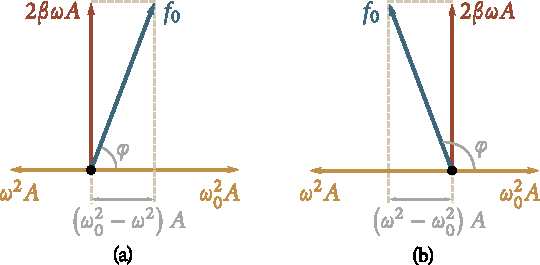
\includegraphics[scale=0.95]{figures/cap_07/fig_7_22.pdf}
		\caption[]{}
		\label{fig:7_22}
	\end{center}
	\vspace{-0.8cm}
\end{figure}

It follows from \eqn{7_123} that the constants $A$ and $\varphi$ must have values such that the harmonic function $f_0\cos\omega t$ will equal the sum of the three harmonic functions in the left-hand side of the equation. If we depict the function $\omega_0^2A\cos(\omega t-\varphi)$ by a vector of length $\omega_0^2A$ directed to the right (\fig{7_22}), then the function $2\beta\omega A\cos(\omega t-\varphi+\pi/2)$ will be depicted by a vector of length $2\beta\omega A$ turned counter-clockwise relative to the vector $\omega_0^2A$ through the angle $\pi/2$ (see Sec.~\ref{sec:7_7}), and the function $\omega^2A\cos(\omega t-\varphi+\pi)$ by a vector of length $\omega_0^2A$ turned through the angle $\pi$ relative to the vector $\omega_0^2A$. For \eqn{7_123} to be satisfied, the sum of the three enumerated vectors must coincide with the vector depicting the function $f_0\cos\omega t$. Inspection of \fig{7_22}a shows that such coincidence is possible only at a value of the amplitude $A$ determined by the condition
\begin{equation*}
	\left(\omega_0^2 - \omega^2\right)^2A^2 + 4\beta^2\omega^2A^2 = f_0^2
\end{equation*}

\noindent
whence,
\begin{equation}\label{eq:7_124}
	A = \frac{F_0/m}{\left[\left(\omega_0^2 - \omega^2\right)^2 + 4\beta^2\omega^2\right]}
\end{equation}

\noindent
(we have replaced $f_0$ with the ratio $F_0/m$). Figure~\ref{fig:7_22}a corresponds to the case when $\omega<\omega_0$. We get the same value of $A$ from \fig{7_22}b corresponding to the case when $\omega>\omega_0$.

Figure~\ref{fig:7_22} also allows us to obtain the value of $\varphi$ showing the lagging in phase of the forced oscillation~\eqref{eq:7_120} behind the driving force producing it. It can be seen from the figure that
\begin{equation}\label{eq:7_125}
	\tan\varphi = \frac{2\beta\omega}{\omega_0^2 - \omega^2}.
\end{equation}

\noindent
Using the values of $A$ and $\varphi$ determined by Eqs.~\eqref{eq:7_124} and~\eqref{eq:7_125} in \eqn{7_120}, we get the function~\eqref{eq:7_119}.

Function~\eqref{eq:7_119} when added to \eqn{7_112} gives the general solution of \eqn{7_111} describing the behaviour of the system upon forced oscillations. Addend~\eqref{eq:7_112} plays an appreciable part only in the initial stage of the process, during the so-called setting in of the oscillations (\fig{7_23}). With the passage of time, owing to the exponential factor $e^{-\beta t}$, the part played by addend~\eqref{eq:7_112} diminishes to a greater and greater extent, and after sufficient time elapses it may be disregarded, retaining only addend~\eqref{eq:7_119} in the solution.

\begin{figure}[t]
	\begin{center}
		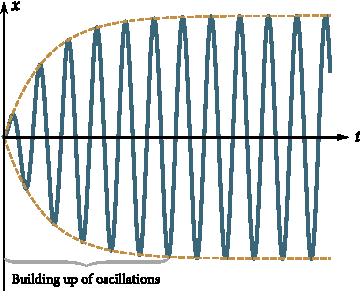
\includegraphics[scale=0.95]{figures/cap_07/fig_7_23.pdf}
		\caption[]{}
		\label{fig:7_23}
	\end{center}
	\vspace{-0.8cm}
\end{figure}

Thus, function~\eqref{eq:7_119} describes steady-state forced oscillations. They are harmonic oscillations with a frequency equal to that of the driving force. The amplitude~\eqref{eq:7_124} of the forced oscillations is proportional to that of the driving force. The amplitude of a given oscillatory system (determined by $\omega_0$ and $\beta$) depends on the frequency of the driving force. Forced oscillations lag in phase behind their driving force; the lagging $\varphi$ also depends on the frequency of the force [see \eqn{7_125}].

As a result of the amplitude of forced oscillations depending on the frequency of the driving force, the amplitude of the oscillations reaches a maximum value at a definite frequency for the given system. The oscillatory system responds especially to the action of the driving force at this frequency. This phenomenon is called \textbf{resonance}, and the corresponding frequency---the \textbf{resonance frequency}.

To determine the resonance frequency $\omega_{\text{res}}$ we must find the maximum of the function~\eqref{eq:7_124} or, which is the same, the minimum of the expression inside the radical in the denominator. Differentiating this expression with respect to $\omega$ and equating it to zero, we get the condition determining $\omega_{\text{res}}$:
\begin{equation}\label{eq:7_126}
	-4\left(\omega_0^2 - \omega^2\right)\omega + 8\beta^2\omega = 0.
\end{equation}

Equation~\eqref{eq:7_126} has three solutions: $\omega=0$ and
$\omega=\pm\left(\omega_0^2-2\beta^2\right)^{1/2}$. The solution equal to zero corresponds to a maximum of the denominator. Of the remaining two solutions, the negative one must be discarded as being deprived of a physical meaning (the frequency cannot be negative). We thus get a single value for the resonance frequency:
\begin{equation}\label{eq:7_127}
	\omega_{\text{res}} = \left(\omega_0^2-2\beta^2\right)^{1/2}.
\end{equation}

\noindent
Using this value of the frequency in \eqn{7_124}, we get an expression for the amplitude in resonance:
\begin{equation}\label{eq:7_128}
	A_{\text{res}} = \frac{F_0/m}{2\beta \left( \omega_0^2 - \beta^2\right)^{1/2}}.
\end{equation}

\noindent
It follows from \eqn{7_128} that the amplitude in resonance would become equal to infinity in the absence of resistance of the medium. By \eqn{7_127}, the resonance frequency in such conditions (at $\beta=0$) coincides with the natural frequency of oscillations of the system $\omega_0$.

The dependence of the amplitude of forced oscillations on the frequency of the driving force (or, which is the same, on the frequency of oscillations) is shown graphically in \fig{7_24}. The separate curves correspond to different values of the parameter $\beta$. According to Eqs.~\eqref{eq:7_127} and~\eqref{eq:7_128}, the peak of a given curve is higher and further to the right with decreasing values of $\beta$. The expression for the resonance frequency becomes imaginary upon very great damping (such that $2\beta^2>\omega_0^2$). This signifies that no resonance is observed in these conditions---the amplitude of forced oscillations monotonously diminishes with increasing frequency (see the lower curve in \fig{7_24}). The curves shown in \fig{7_24} corresponding to different values of the parameter $\beta$ are called \textbf{resonance curves}.

\begin{figure}[t]
	\begin{center}
		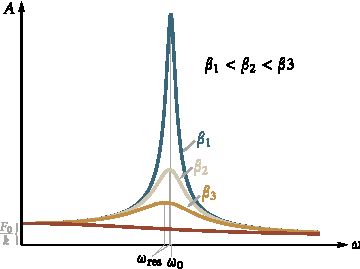
\includegraphics[scale=0.95]{figures/cap_07/fig_7_24.pdf}
		\caption[]{}
		\label{fig:7_24}
	\end{center}
	\vspace{-0.8cm}
\end{figure}

We can add the following remarks with respect to resonance curves. When $\omega$ tends to zero, all the curves arrive at the same limiting value equal to $F_0/(m\omega_0^2)$, \ie, $F_0/k$, differing from zero. This value is the displacement from the equilibrium position received by the system under the action of a constant force of magnitude $F_0$. When $\omega$ tends to infinity, all the curves asymptotically tend to zero because at a high frequency the force changes its direction so rapidly that the system does not manage to become displaced from its equilibrium position. Finally, we must note that diminishing of $\beta$ is attended by a greater change in the amplitude with the frequency near resonance and by a sharper ``peak''.

It follows from \eqn{7_128} that with small damping (\ie, when $\beta\ll\omega_0$), the amplitude in resonance is
\begin{equation*}
	A_{\text{res}} \approx \frac{F_0/m}{2\beta\omega}.
\end{equation*}

\noindent
Let us divide this expression by the displacement $x_0$ from the equilibrium position under the action of the constant force $F_0$ equal to $F_0/(m\omega_0^2)$. The result is
\begin{equation}\label{eq:7_129}
	\frac{A_{\text{res}}}{x_0} \approx \frac{\omega_0}{2\beta} = \frac{2\pi}{2\beta T} = \frac{\pi}{\lambda} = Q
\end{equation}

\noindent
[see \eqn{7_106}]. Thus, the quality $Q$ shows how many times the amplitude at the moment of resonance exceeds the displacement of the system from its equilibrium position under the action of a constant force of the same magnitude as the amplitude of the driving force (this holds only with slight damping).

\begin{figure}[t]
	\begin{center}
		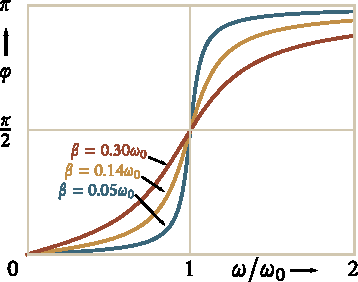
\includegraphics[scale=0.95]{figures/cap_07/fig_7_25.pdf}
		\caption[]{}
		\label{fig:7_25}
	\end{center}
	\vspace{-0.8cm}
\end{figure}

Inspection of \fig{7_22} shows that forced oscillations lag in phase behind their driving force; this lagging ranges from $0$ to $\pi$. The dependence of $\varphi$ on $\omega$ at various values of $\beta$ is shown in \fig{7_25}. The value $\varphi=\pi/2$ corresponds to the frequency $\omega_0$. The resonance frequency is lower than the natural one [see \eqn{7_127}]. Hence, at the moment of resonance, $\varphi<\pi/2$. When the damping is insignificant, $\omega_{\text{res}}\approx\omega_0$, and we may assume that in resonance $\varphi=\pi/2$.

The phenomenon of resonance must never be forgotten in designing machines and various structures. The natural frequency of oscillations of such equipment and facilities must not be close to the frequency of possible external actions. For example, the natural frequency of vibrations of a ship's hull or an aeroplane's wings must greatly differ from the frequency of the vibrations that might be produced by rotation of the propeller. Otherwise vibrations will appear that may cause a catastrophe. Cases are known when bridges collapsed owing to the marching of columns of soldiers over them. The reason was that the natural frequency of oscillations of the bridge was close to the frequency of the soldier's steps.

The phenomenon of resonance, at the same time, is often very useful, especially in acoustics, radio engineering, etc.

\section{Parametric Resonance}\label{sec:7_13}

In the case dealt with in the preceding section, a driving force applied from outside produced a direct displacement of a system from its equilibrium position. Another kind of external action is known to exist by means of which great oscillations can be imparted to a system. This kind of action consists in periodically changing a parameter of the system in step with its oscillations, owing to which the phenomenon is called \textbf{parametric resonance}.

\begin{figure}[t]
	\begin{center}
		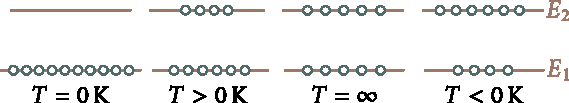
\includegraphics[scale=0.95]{figures/cap_07/fig_7_26.pdf}
		\caption[]{}
		\label{fig:7_26}
	\end{center}
	\vspace{-0.8cm}
\end{figure}

Let us take as an example a simple pendulum---a ball on a thread. If we periodically change the length $l$ of the pendulum, increasing it when the pendulum is at its extreme positions and decreasing it when the pendulum is at its middle position (\fig{7_26}), then the pendulum starts swinging violently. The energy of the pendulum here grows at the expense of the work done by the force acting on the thread. The force tensioning the thread is not constant when the pendulum oscillates: it is smaller at the extreme positions when the velocity vanishes, and is greater at the middle position when the velocity of the pendulum is maximum. Consequently, the negative work of the external force upon elongation of the pendulum is smaller in magnitude than the positive work done upon shortening of the pendulum. As a result, the work done by the external force during a period is greater than zero.

